\section{Architecture Overview}
\label{section:architecture_overview}

The model presented in Figure~\ref{fig:model} organises all the components involved in this system, considering a scenario where an embodied agent plays a physical card game against human players over a touch table.

\begin{figure}[ht]
  \centering
    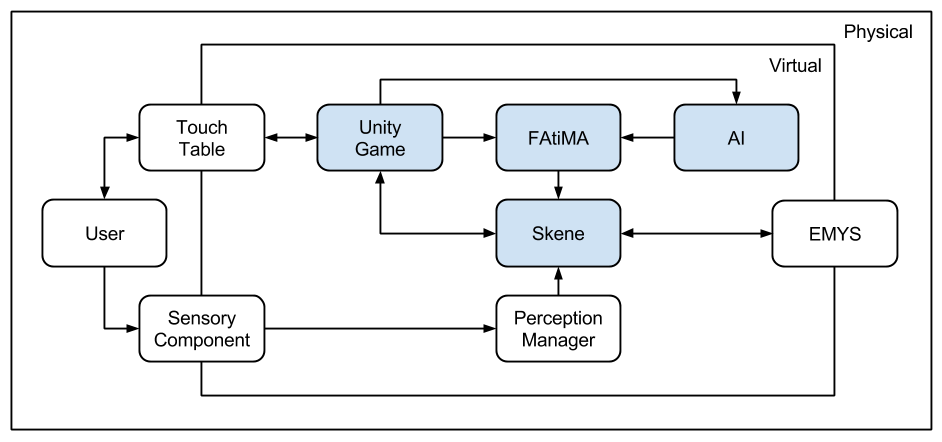
\includegraphics[width=1\textwidth]{./img/model}
  \caption{Structure of the social robot that plays \emph{Sueca}}
\label{fig:model}
\end{figure}

This model distinguishes physical components from virtual ones.
Some entities are not detailed on the scope of this project and are presented as both physical and virtual components.
The human players, Users, play with physical cards on top of a Touch Table, and their game actions are managed by Game Application and communicated to both the \ac{ai} module and the Decision Maker.
The Perception Manager receives information from all the Sensory Components.
The \ac{ai} module includes all the reasoning about the game and decides the robot's next move.
However, the embodied agent's actions also involve social behaviours, and Decision Maker is the responsible module for this management.
The Decision Maker balances the \ac{ai} move and game information, depending on the situation, in order to produce an appropriate sequence of behaviours and inform them to Behaviour Planner.
For instance, being the last player of a trick and taking the two highest cards of a suit, by playing a trump card, is an exciting move and should produce an equally exciting reaction on the robot.
Lastly, the Behaviour Planner, after receiving high-level intention-directed instructions, builds a suitable plan to execute the chosen instructions, considering the state of the embodied agent, information from Perception Manager, and additional game information from the Game Application.

The architecture that will instantiate the model described above is partially decided.
The virtual layer will be mainly covered by Thalamus framework, which enables the communication between the mentioned entities \cite{Ribeiro}.
The chosen Behaviour Planner is Skene \cite{Ribeiroa}.
The \ac{ai} module will be processed offline with the algorithms described in Section~\ref{sec:sueca_solution}.
The embodied agent will initially be \ac{emys} due to its expressiveness, although other robots will be considered, depending on the users' preferences.
Finally, the undecided components are the sensory inputs.
Since Pereira et al. have shown the importance of collecting data from user studies, these components will be settled further, after some field research with \emph{Sueca} players.